\documentclass{standalone}
\usepackage[T1]{fontenc}
\usepackage[latin2]{inputenc}
\usepackage[english]{babel}
\usepackage{tikz}
\usetikzlibrary{calc,through,backgrounds,positioning,fit}
\usetikzlibrary{shapes,arrows,shadows}
 
\begin{document}
 
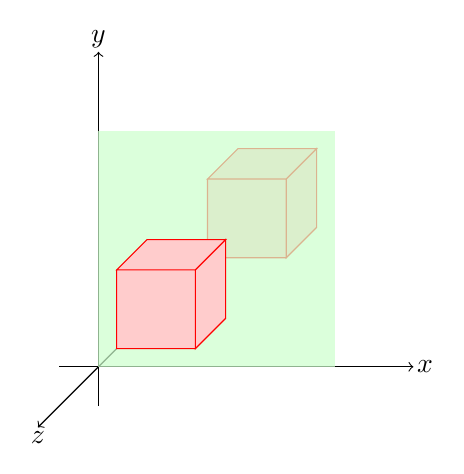
\begin{tikzpicture}[scale=1,inner sep=0.4mm]
\coordinate (A) at (2,2,2);
\coordinate (B) at (2,2,-1);

\draw [->] (0,0,-1) -- (0,0,2) node [below] {$z$};
\draw [->] (0,-.5,0) -- (0,4,0) node [above] {$y$};
\draw [->] (-.5,0,0) -- (4,0,0) node [right] {$x$};
\filldraw [draw=red,fill=red!20!white] 
  (B) -- ++(0,-1,0) -- ++(-1,0,0) -- ++(0,1,0) -- cycle
  (B) -- ++(0,-1,0) -- ++(0,0,-1) -- ++(0,1,0) -- cycle
  (B) -- ++(-1,0,0) -- ++(0,0,-1) -- ++(1,0,0) -- cycle;
  
\fill [fill=green!20!white, opacity=0.7]  (0,0,0) -- (3,0,0) -- (3,3,0) -- (0,3,0) -- cycle;
  
\filldraw [draw=red,fill=red!20!white] 
  (A) -- ++(0,-1,0) -- ++(-1,0,0) -- ++(0,1,0) -- cycle
  (A) -- ++(0,-1,0) -- ++(0,0,-1) -- ++(0,1,0) -- cycle
  (A) -- ++(-1,0,0) -- ++(0,0,-1) -- ++(1,0,0) -- cycle;
% płaszczyzna symetrii, osie x i y, druga kostka

\end{tikzpicture}
 
\end{document}